\chapter{Dias}		% chapter 1
\label{codechap}
\section{Dias}

\subsection{Monte Carlo Simulator}
{\sc dias} (Dynamics In Artificial Solids) is a code which at its heart is a Monte-Carlo simulator. {\sc dias} begins by taking in parameters such as granule-to-granule distance, number of electrons, number of lattice sites, number of time-steps, temperature, voltage bias, thermal gradient, material coefficient, and substrate potential variance. The granule-to-granule distance is on the order of 10 nanometeres. We have a square grid which is periodic. Variances in granule distances are uniformly introduced with limits according to user-set parameters. The number of electrons can vary between double-empty systems and double occupied sites. The number of time-steps is usually set to the square of the number of particles. This is to ensure a statistically justified result from the monte carlo aspect of the simulation. Temperature is set in Kelvin and is usually varied in the range where our material coefficient would give interesting results.  A positive voltage bias will act on a particle so that it is coerced to move upstream. Conversely, a positive voltage bias will force a hole to move downstream. This hints at a particular symmetry in which we chose for the simulation. Some previous studies have chosen to only focus on electron jumps and reject any jump that begins with a hole ~\cite{Ferrero14}. We decided to allow jump probabilities to be calculated from an electron hole's point of view as well. For current/voltage measurements, the system is periodic so that the current will just keep traveling at a steady pace. The code was also forked to a closed system to study thermoelectric properties. The memory choices we made are also worth mentioning. There were several arrays of data and keeping these to a minimum was important as memory management was an issue due to the limited space on GPU cards. We had between 1.5 and 2 Gb of memory to work with. These matrices include particle/hole, substrate potential, distance between sites, thermal gradient, and size of each granule. In order to maintain neutrality, the voltage bias was artificially set. This meant that the effective charge of a filled site was half an electron. If an electron were to move, the charge then became negative half and electron. The Monte-Carlo algorithm shows up twice to find the jump site.  First, a lattice site is chosen with probability according to it's energy. Second, the jump probabilities to each site are calculated using Eq.~\ref{probability} for said site. These probabilities are summed up and a number is chosen between 0 and that sum. This in turn gives a Monte-Carlo jump which is weighted by the jump probabilities. This jump is done and the system moves on to the next timestep under the new electron configuration. Meanwhile the properties of interest are measured. This repeats for the number of requested time steps. The pseudocode describing this process was outlined below:

\begin{varwidth}{\dimexpr\linewidth-2\fboxsep-2\fboxrule\relax}
\begin{algorithmic}[1]
\State Total = 0
\For {i = 1 to number of sites}
\State Total =+ $W_i$
\EndFor
\State newSum = 0
\State pick a random number R from 0 to Total
\For {i = 1 to number of sites}
\State newSum =+ $W_i$
\If {newSum $>$ R}
\State stop For loop, that is the jump site
\EndIf
\EndFor

This pseudocode is what is referred to as the "Tower Method". It is used in picking the starting particle as well as picking the particle to jump to. 
\end{algorithmic}
\end{varwidth}%

Originally we picked the starting particle randomly. Unfortunately in order to have a rejection-less system, this cannot happen. If it did, then particles which would have practically no chance of jumping would be moved with probability $ 1/N^2$. In order to fix this, we followed the algorithm posed in ~\cite{Newman99}. They propose first picking two particles with probabilities via the tower method,based on their energies. This way, particles which are less stable are moved more often. Because of the distance parameter in our probability, we are forced to pick one particle at a time. This way the second particle is picked based on the change of energy of the system, with a distance component. This algorithm allows for maximum parallelization and no rejection. The parallelized tower method is efficient as we can use a parallel prefix scan to stack the probabilities while also finding the maximum value in order to normalize. Doing a search for the right interval can also occur in parallel as each thread can be given a range, and the appropriate range can be found in log(N) time. 

\begin{varwidth}{\dimexpr\linewidth-2\fboxsep-2\fboxrule\relax}
\begin{algorithmic}[1]
\State number of slices = sizeArray/sharedMemory + 1
\State size of slice = sharedMemory
\State sumStart = 1
\For {i = 1 to number of slices}
\For {k = 1 to log(size of slice)}
\For { j = sumStart to size of slice/2}
\State add first half of slice to second half, put that sum in the second half
\EndFor
\State sumStart = size of slice/2
\State size of slice  = size of slice / 2
\EndFor
\EndFor
\State (now we stitch each shared memory together)
\State totalSum = 0
\For {i = 1 to number of slices}
\State totalSum = totalSum + sliceSum
\EndFor

This pseudocode is what is referred to as the "Parallel Reduction". It is device specific to GPGPU's, but can be generalized depending on "shared memory". This can be easily combined with a simple parallel sum to create a parallel dot-product algorithm. 
\end{algorithmic}
\end{varwidth}%

\subsection{Conditions}
There are certain conditions which an algorithm must comply with in order to be considered a Markov Chain Monte Carlo. The first is that the probability function should not vary over time. That is clearly satisfied as we stay in the form:

\begin{eqnarray}
P = e^{-2R - \Delta E/T},
\label{simpleProb}
\end{eqnarray}
where the probability of jumping is a function of the jump distance $r$, change in energy of the system $E$, and temperature of the jump site $T$. The second is that the probability to jump to the next state is only a function of the current state. In other words, there is no "momentum" built up from previous states. Third is that the sum of the probabilities must equal 1: 
\begin{eqnarray}
\Sigma P(\mu \rightarrow \nu) = 1 ,
\label{normalized}
\end{eqnarray}
Where $\mu$ is the current state and this is being summed over all possible transitions to other states $\nu$. Fourth is the requirement of ergodicity. That is, all states should be reachable from all other states given enough time. This requirement is satisified as long as there is at least one non-zero probability to jump out of every other state. Finally, our last condition is of detailed balance. That is upon relaxation we generate the Boltzmann probability distribution rather than any other.

\subsection{Thoon Cluster}
This research was performed on a variety of machines, mostly consisting of Nvidia graphics cards. I had access to one stand-alone pc with a GTX 570, 8 pcs in a computer lab with GTX 570s, and 60 nodes with 2 GPU's each on the Gaea cluster in the computer science building. The Gaea cluster was powerful, but frequently busy such that only a third to an eighth was typically available. Meanwhile there was a computer lab with 8 linux based pcs, each with an Nvidia gtx 570. Unfortunately, they were barely on the same network. To remedy this, I wrote a script which divided up the parameter scans in the form of bash scripts and sent these to the respective computers. These then started the simulations and a timer in the form of a cron argument. The cron would then check every five minutes to see if the simulation was done. If so, then the data was sent back to the host computer. This had a few weaknesses, namely the clunkyness and the fact that one had to wait for the cron to trigger. This meant that short scans were impractical. Eventually this was all replaced with the free-lisence version of the Torque job scheduler. With the computers united into a small "cluster", running batches became more streamlined. This ad-hoc cluster is called THOON (Torque Hub On One Node). 

\subsection{GPU Algorithms}
The problem of electron hopping via Monte-Carlo algorithm can be solved very efficiently using parallel/GPU algorithms. In particular we use an algorithm called the "tower method" ~\cite{Krauth06}. Typically when one is doing a Monte Carlo study, there is an acceptance region and a rejection region ammong a range of choices. A choice is examined and it is either rejected or accepted. Using the tower method, all choices are stacked on top of each other (like a tower) and there is no rejection region. The first step, finding the probability to jump to each site is solved via the classical parallel scheme, where each lattice site can be individually calculated in its own thread. Once we have the probability matrix, we need to sum it in order to normalize it. This can be done via a parallel reduction algorithm. Taking advantage of on-board GPU memory, we can perform the reduction in O(N/P + log N ) time rather than O(N) time, where P is the number of GPU cores. Now that the system is normalized, we can roll a dice between 0 and 1 to find where the particle will go. We must then sum our probabilities until we find that number. This can be done with a parallel prefix sum. Parallel reduction and prefix sum algorithms were written and then replaced by Nvidia's more efficient Thrust functions. Thrust is a template library for CUDA which allows the implementation of high performance parallel applications.

\begin{varwidth}{\dimexpr\linewidth-2\fboxsep-2\fboxrule\relax}
\begin{algorithmic}[1]
\State First a nearest neighbor exchange
\For {i = 1 to number of sites}
\If {there's a particle at that site}
\State calculate energy without moving the particle:
\State {\textit{potential energy calculated everywhere}}
\State {\textit{sum reduction of the potential energy to one number (lets call it $S_1$) }}
\State test moving the particle up
\State {\textit{potential energy calculated everywhere}}
\State {\textit{sum reduction of the potential energy to one number (lets call it $S_2$) }}
\If {$S_1$ $>$ $S_2$}
\State leave the system
\Else
\State change it back
\EndIf
\State repeat for the other 3 directions (down,left,right)
\EndIf
\EndFor
\State The system is now slightly more relaxed
\State Now for switching highs and lows
\While {system is not relaxed}
\For {j = 1 to number of sites}
\State find the energy at each site normally:
\State {\textit{calculate potential,substrate, \& coulomb blockade energy everywhere. Sum and call this $S_3$}}
\State find the energy at each site with the particle removed (or added if the site was empty ):
\State {\textit{calculate potential,substrate, \& coulomb blockade energy everywhere. Sum and call this $S_4$}}
\State DosMatrix[j] = $S_4$ - $S_3$
\EndFor
\State {\textit{find lowest and highest values on the DosMatrix}}
\If {DosMatrix[index of lowest] + DosMatrix[index of highest] $<$ 0 }
\State swap particles
\Else
\State system is relaxed
\EndIf
\EndWhile
\end{algorithmic}
\end{varwidth}%

\subsection{Optimizations}
Various optimizations were done in order to speed up this code. Originally this was a linear CPU code, but obvious parallelisms made this code perfect for being run on a GPU. Still, there were some less obvious optimizations. One such optimization was previously discussed, moving to a rejection free system. In a rejection system, the particle has a high chance of staying at the same cell each turn. This means that a lot of computation is spent not gaining any valuable information. To fix this, we moved to the rejection free system (BLK?)~\cite{Newman99}. It is as if one jumped the simulation forward skipping all non-events. For one to do this, the system time must be kept. This is done by integrating all of the probabilities:
\begin{eqnarray}
\delta t = \frac {1} {\Sigma P_{\mu \rightarrow \nu}},
\label{systemTime}
\end{eqnarray}
where $\delta t$ is the change in system time, and $P_{\mu \rightarrow \nu}$ is the Markov transition matrix. Because of {\sc cuda} and algorithms like parallel reductions, it ends up being much faster to calculate this than to try to calculate all of the rejections. There were optimizations that skipped unnecessary calculations. One of these was the calculation of the potentials after a particle is moved. The naive way to do this would be to recalulate all of the potentials from each particle. The optimized way to do this would be to use a crater-mound system. That is, only focus on the effects due to the particle that has moved. In other words, add a crater to the potential around the site where a particle left and add a mound in the potential around the site where the particle has appeared. Another optimization was the 4D lattice matrix. 

\subsection{The Lattice}
While the easiest system to model would have been a square lattice, This would have left out a large amount of interesting phenomena. To incorporate this, we started out with a square lattice and then gave each site a certain $\delta x$ or $\delta y$ variance. There are a few ways to then use this kind of implementation. The first one would have been to then calculate the distances from one site to another on the fly, possibly approximating for further away site. The way that we picked to do this was to hold all of the distances from one site to another in a 4D matrix (a matrix of distances for every site on the grid). This has the advantage that no calculations have to be run at each GPU core. Since the calculation of distance involves a square root, this would have been heavy on the workload. The disadvantage is that for a $100 \times 100 $ system, we require $100 \times 100 \times 4$ bytes of data (or 400MB using the float type). Fortunately, NVIDIA GTX 570 cards have at least 1200 megabytes of memory, so this did not end up being an issue.

\subsection{Dielectric Constant}
We also varied the dielectric constant of the material. Typical dielectric constant was held at around 4. For gold nanoparticles, this number can increase. While gold is a conductor and conductors tend to have a dielectric constant of infinity, these gold nano-particles are in very special situation. First, they are small, so there are skin-level effects which mean that while the interior may want to reach a high dielectric constant, the skin still has a finite constant. Second, The dielectric constant of gold varies with frequency. It may be infinite for a static field attempting to permeate through a block of gold, but different frequencies will feel different impedances.  

\subsection{Distance-substrate correlation}
In the physical world, this system is not a grid, but rather a dense packing of granules. This can be imagined as a 2D packing of variously sized orbs. One can then see that the distance between orb centers will depend on the size of the neighboring orbs. For ease of algorithms, we took this correlation in the opposite direction. The size of an orb is defined by half the distance to the nearest orb. The substrate potential is also affected by this. Granule size randomness did not have much effect on the system directly. This is because it only affects how much energy it takes to pack two electrons on the same granule. If the granule is bigger, the electrons do not have to sit so close together and the charging energy is lowered. But the issue is that even with a larger granule, the temperature required to pack two electrons onto the same granule is still in the thousands of Kelvin and outside of the scope of this study. The correlation's effect on substrate randomness however did come into effect, as small changes in the substrate potential can have large effects on the density of states.

\subsection {Density of States}
The energy involved when removing or adding a particle to a lattice site is what determines the probability to jump to it. It then makes sense to ask what the distribution of potential energies will be. The purpose of this code was not originally to determine the density of energy states of an electron lattice. Nevertheless it serves two practical purposes. First, it helps to make sure that the particular energy contributions are balanced accordingly. Looking at the density of states, one can immediately associate characteristics to electrical potential, substrate potential, etc. Then, at a glance, one can quickly determine if the substrate potential is too strong and is washing out electric potential contributions. The second purpose is to assure that a particular system is fully relaxed before simulations begin. Due to the inherent randomness of the system, particular outcomes may sharply vary depending on the initial conditions. Assuring that the system is relaxed before starting can compensate for this. One clue that the system is relaxed is that in two dimensions, there will be a linear (absolute value) pattern near 0 in the density of states. We use a previously determined algorithm in order to quickly relax our system ~\cite{Vinokur08}. We begin with a nearest-neighbor comparison of every particle site and moving them if the overall energy is lower. Then we find the particle which is imparting the most potential energy by existing. This is compared to the hole for which filling it would cause the most potential energy to be added to the system. If the two energies, when summed, are less than the original, then the switch is performed. The area around each switched particle is then scanned to see if any readjustments can be made to further lower the potential energy of the system. The density of states is then measured again everywhere and the process is repeated until the energy can no longer be reduced. The valley in the density of states can also be characterized. If the slope near $E=0$ is linear, then we know we are looking at a 2D system. If it is parabolic, then this signifies a 3D system. As a benchmark, we analyzed our valley slope and found it to agree with the 2D system characterization. 

\subsection{Algorithmic Benchmarking}
The average jump distance for a high temperature system should be ~0.69614 spaces. This matches to within $1\%$ accuracy with my results of 0.68943 spaces. This difference is negligible considering the statistical variation of any Monte Carlo system. The expected jump distance was found via Monte Carlo integrator. First, the values of Eq.~\ref{probability} were found at a grid of points with similar spacing to what we use in the simulation. Second, particles were dropped onto this grid depending on the function values a-la Monte Carlo method. Third, the mean jump distance was calculated via the first moment equation
\begin{eqnarray}
\bar r = \frac {\sum r \cdot n} {\sum n}, 
\label{firstMoment}
\end{eqnarray}
where $r$ is the distance from the center of the grid cell, and $n$ is the number of particles at each grid cell. The parameters for this comparison were fairly basic. The temperature was 1 degree kelvin, there was no external current, the system size was 100x100, and there was only one particle. Multiple particle comparisons have been done, but because the jump probabilities are different depending on wether the site is empty or full, the comparison becomes much more complicated. The point of this benchmark was to make sure the complicated GPU Monte-Carlo integrator was working as expected. With 3 major components to this system, (calculating the energies, calculating the weights from the energies, and calculating a jump site from the weights), this was a simple way to make sure everything was working together properly. Creating simple scripts to test more complicated scripts also became a useful tool in other parts of the research. For example, studying the behavior of the energy as a function of distance can be done via the Dias simulator, and outputs can be output for testing. But this can be complicated and the program may need to be changed and re-compiled in between tests. By writing a simple function grapher in Octave and tuning the same parameters, the interaction between different energy sources could be observed more closely.

\subsection{Results}
  Other results also followed the expected trends. In Fig.~\ref{TvsRbar} , One can see that as the temperature rises, the system slowly kills any aditional help from the $E_{ij}$ component and it asymptotes to the jump distance related to the locality of the electron. In Fig.~\ref{JvsV} , The dependance of current on voltage is almost exponential. In Fig.~\ref{TvJ}, one can see how the electrons can't go as far once the temperature is increased. A modified version of the simulator was run to explore the physics of electron transport as the system becomes saturated. The number of electrons in the system was slowly increased and simulations were run at different numbers of particles. In ~\cite{Beloborodov07} they give approximate jump distances at various temperatures. We duplicated these and found similar values for $\bar \mu = .01$ and $\delta xy = .45$.

\begin{figure}[htbp]
\begin{center}
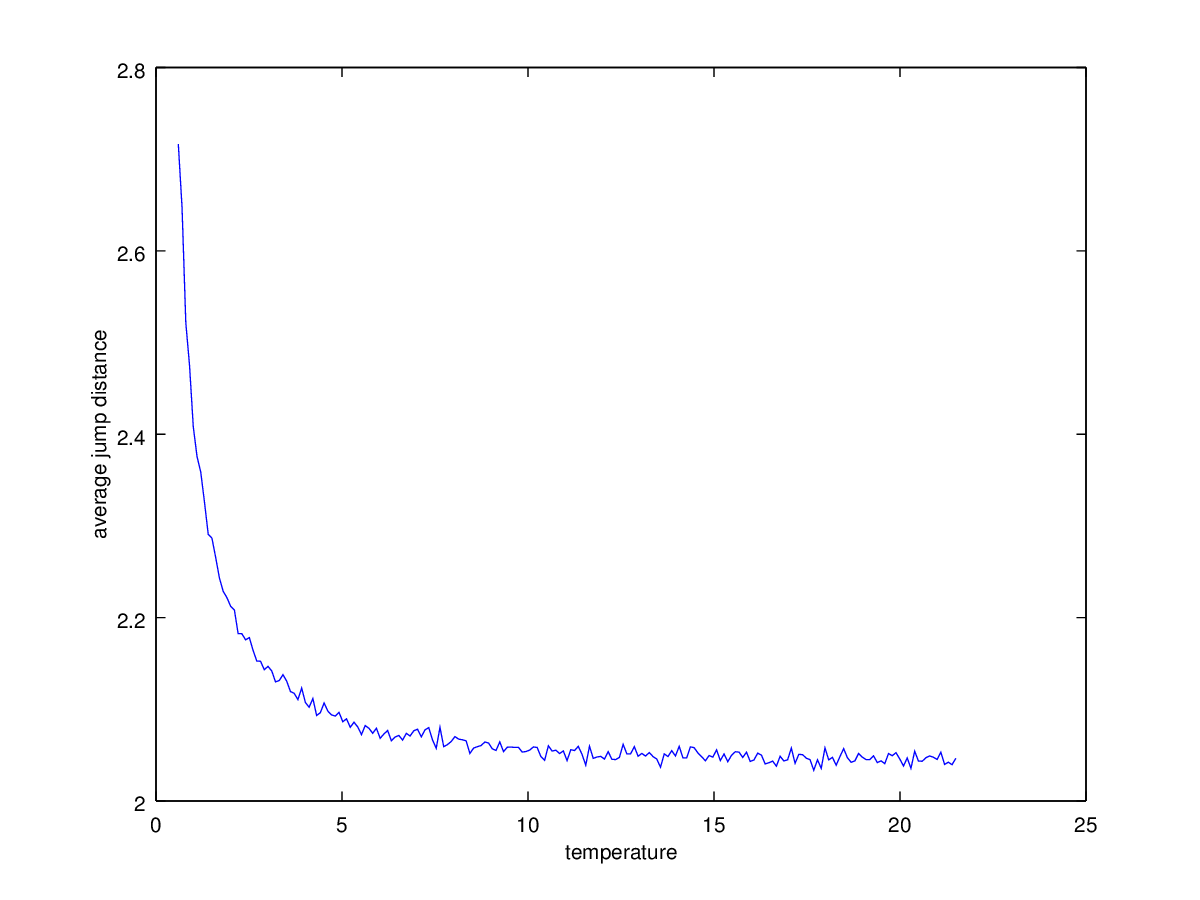
\includegraphics[scale=.50]{TvsRbar.png}
\caption{Temperature vs average jump distance .}
\label{TvsRbar}
\end{center}
\end{figure}

\begin{figure}[htbp]
\begin{center}
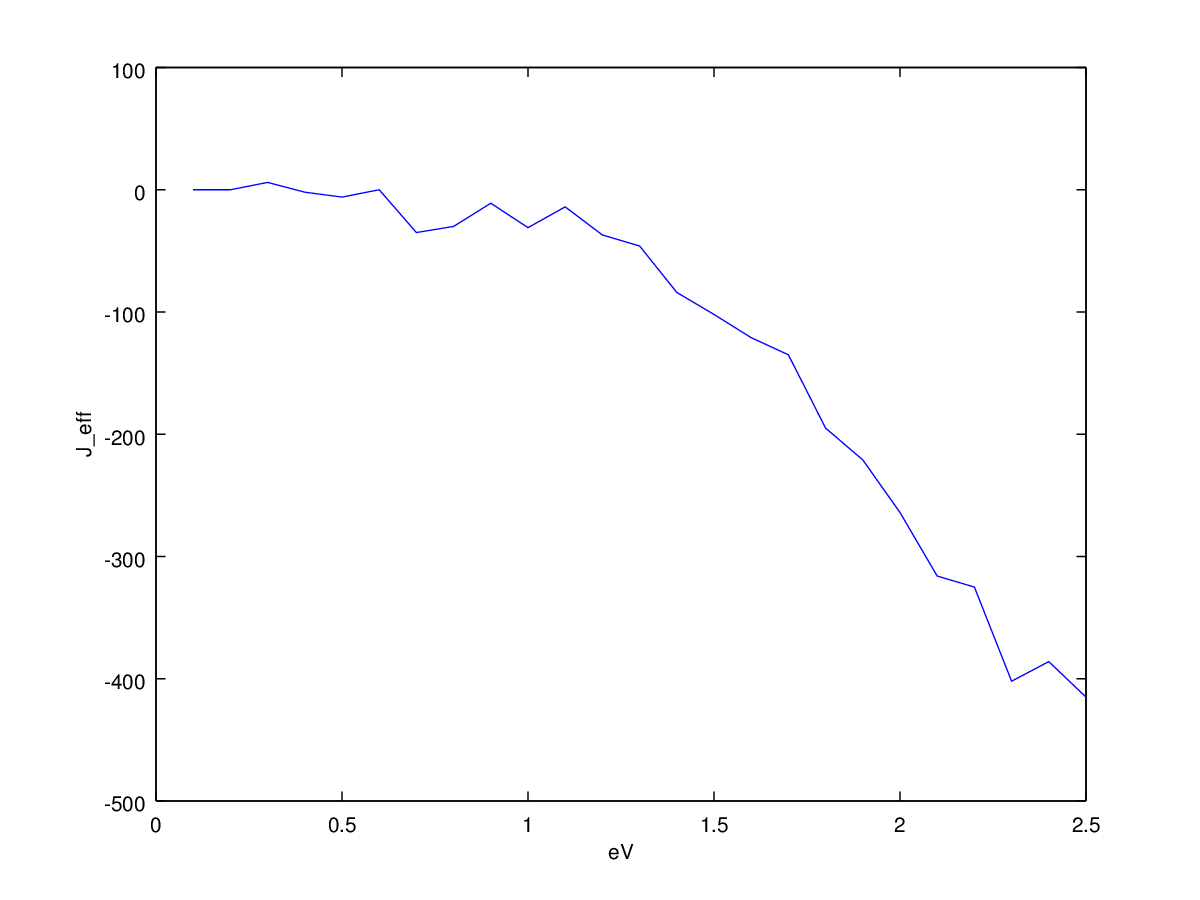
\includegraphics[scale=.50]{JvsV.png}
\caption{Current vs Voltage .}
\label{JvsV}
\end{center}
\end{figure}

\begin{figure}[htbp]
\begin{center}
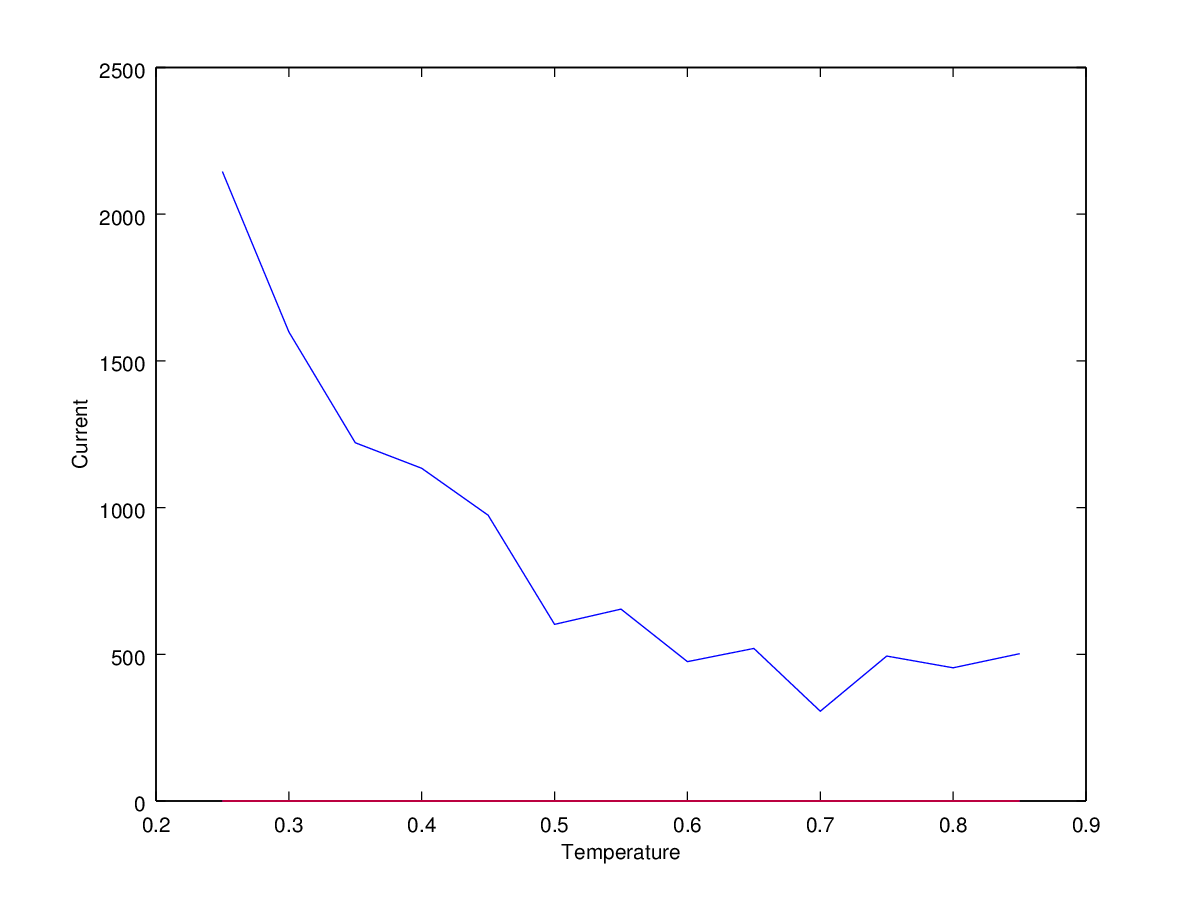
\includegraphics[scale=.50]{JvT.png}
\caption{Temperature vs current .}
\label{TvJ}
\end{center}
\end{figure}

